\documentclass[aspectratio=169]{beamer}

\usepackage[T1]{fontenc}
\usepackage{amsmath}
\usepackage{amssymb}
\usepackage{graphicx}
\usepackage{tikz}
\usepackage{booktabs}
\usepackage[autostyle]{csquotes}
\MakeOuterQuote{"}
\usetikzlibrary{arrows.meta, positioning, calc}

\definecolor{coolpurple}{HTML}{7f65a0}
\definecolor{lightpurple}{HTML}{ede8f5}
\definecolor{darktext}{HTML}{1a1a2e}
\definecolor{highlightpurple}{HTML}{5a3e82}

\setbeamercolor{normal text}{fg=darktext, bg=white}
\setbeamercolor{structure}{fg=coolpurple}
\setbeamercolor{frametitle}{fg=white, bg=coolpurple}
\setbeamercolor{title}{fg=white, bg=coolpurple}
\setbeamercolor{subtitle}{fg=white}
\setbeamercolor{date}{fg=coolpurple}
\setbeamercolor{author}{fg=coolpurple}
\setbeamercolor{item}{fg=coolpurple}
\setbeamercolor{subitem}{fg=coolpurple!70!black}
\setbeamercolor{block title}{bg=coolpurple, fg=white}
\setbeamercolor{block body}{bg=lightpurple, fg=darktext}
\setbeamercolor{alerted text}{fg=highlightpurple}

\setbeamertemplate{itemize item}{\color{coolpurple}$\blacktriangleright$}
\setbeamertemplate{itemize subitem}{\color{coolpurple!70}$\bullet$}
\setbeamertemplate{navigation symbols}{}
\setbeamertemplate{footline}{%
	\hfill\insertframenumber\,/\,\inserttotalframenumber\hspace{1em}\vspace{0.5em}
}

\newcommand{\hl}[1]{\textcolor{coolpurple}{\textbf{#1}}}
\newcommand{\R}{\mathbb{R}}
\newcommand{\xn}[1]{x^{(#1)}}
\newcommand{\eps}{\hat\varepsilon}

\graphicspath{{../../results/}}

\title{BendFlow: Where Flow Matching Trajectories Bend}
\subtitle{Project proposal, Visual Generative Models}
\author{Lado Turmanidze \and Geronimo Castaño}
\institute{\small{Universit\"at des Saarlandes}}
\date{December 2, 2026}

\begin{document}

	\begin{frame}
		\titlepage
	\end{frame}

	\begin{frame}{Sampling Is Following A Path}
		\begin{columns}[onlytextwidth, T]
			\begin{column}{0.52\textwidth}
				\small
				\begin{itemize}
					\item \hl{Flow matching} generates an image by following a velocity field from noise ($t = 0$) to data ($t = 1$).
					\vspace{0.4em}
					\item \hl{In practice} the path is followed with a few Euler steps: look at the direction, walk straight, repeat.
					\vspace{0.4em}
					\item \hl{Where the path is straight}, a large step loses nothing. \hl{Where it bends}, a large step lands in the wrong place.
				\end{itemize}
			\end{column}
			\begin{column}{0.44\textwidth}
				\centering
				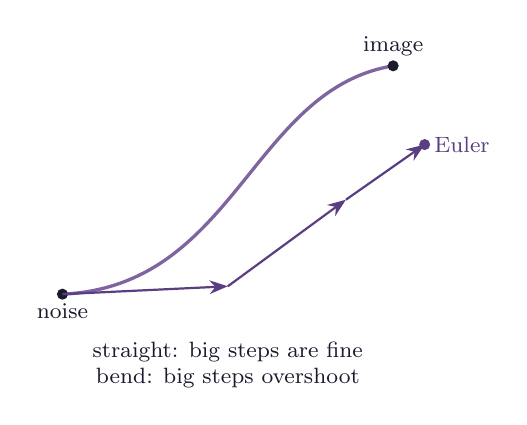
\begin{tikzpicture}[scale=1.0]
					\draw[very thick, coolpurple] (0,0) .. controls (2.2,0.1) and (2.4,2.6) .. (4.2,2.9);
					\fill[darktext] (0,0) circle (2pt) node[below, font=\footnotesize] {noise};
					\fill[darktext] (4.2,2.9) circle (2pt) node[above, font=\footnotesize] {image};
					\draw[thick, highlightpurple, -{Stealth}] (0,0) -- (2.1,0.1);
					\draw[thick, highlightpurple, -{Stealth}] (2.1,0.1) -- (3.6,1.2);
					\draw[thick, highlightpurple, -{Stealth}] (3.6,1.2) -- (4.6,1.9);
					\fill[highlightpurple] (4.6,1.9) circle (2pt) node[right, font=\footnotesize] {Euler};
					\node[font=\footnotesize, text=darktext, align=center] at (2.1,-0.9) {straight: big steps are fine\\ bend: big steps overshoot};
				\end{tikzpicture}
			\end{column}
		\end{columns}
		\vspace{0.8em}
		\begin{center}
			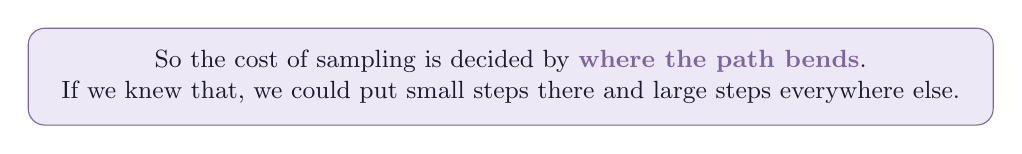
\begin{tikzpicture}
				\node[draw=coolpurple, fill=lightpurple, rounded corners=6pt, inner xsep=12pt, inner ysep=8pt, align=center, font=\small, text=darktext] {So the cost of sampling is decided by \textcolor{coolpurple}{\textbf{where the path bends}}.\\ If we knew that, we could put small steps there and large steps everywhere else.};
			\end{tikzpicture}
		\end{center}
	\end{frame}

	\begin{frame}{How Is "Where Is It Hard?" Answered Today?}
		\begin{block}{Current answers (e.g. CSFlow, Stable Velocity, 2026)}
			\small Find a \hl{range of timesteps} where the field is hard to learn or to follow, for each dataset, and spend more training or more sampling steps there.
		\end{block}
		\vspace{0.4em}
		\begin{columns}[onlytextwidth, T]
			\begin{column}{0.48\textwidth}
				\begin{block}{What this does not say}
					\small
					\begin{minipage}[t][2.4cm][t]{\linewidth}
						\begin{itemize}
							\item \emph{why} these timesteps are hard
							\item anything about a \emph{single} sample: every sample gets the same schedule
						\end{itemize}
					\end{minipage}
				\end{block}
			\end{column}
			\begin{column}{0.48\textwidth}
				\begin{block}{The question of this project}
					\small
					\begin{minipage}[t][2.4cm][t]{\linewidth}
						For \hl{one sample}, at \hl{one moment}: what makes its path bend, and can we read that off from quantities the sampler already computes?
					\end{minipage}
				\end{block}
			\end{column}
		\end{columns}
	\end{frame}

	\begin{frame}{The Idea: Difficulty Is Indecision}
		\begin{columns}[onlytextwidth, T]
			\begin{column}{0.55\textwidth}
				\small
				\begin{itemize}
					\item At every noisy point the model implicitly answers: \hl{which training image did this come from?}
					\vspace{0.3em}
					\item The answer is a probability distribution over training images, the \hl{posterior}.
					\vspace{0.3em}
					\item \hl{Claim:} the path bends while the posterior is still split between images that are far apart, and it is straight once it has \hl{committed} (put almost all its weight on one image).
				\end{itemize}
			\end{column}
			\begin{column}{0.41\textwidth}
				\centering
				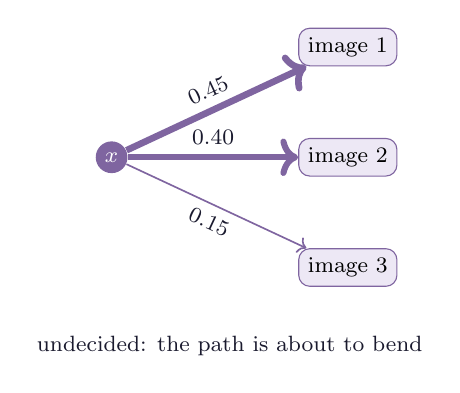
\begin{tikzpicture}[font=\footnotesize]
					\node[circle, fill=coolpurple, text=white, inner sep=2pt] (x) at (0,0) {$x$};
					\node[draw=coolpurple, fill=lightpurple, rounded corners] (a) at (3,1.4) {image 1};
					\node[draw=coolpurple, fill=lightpurple, rounded corners] (b) at (3,0) {image 2};
					\node[draw=coolpurple, fill=lightpurple, rounded corners] (c) at (3,-1.4) {image 3};
					\draw[->, line width=2.4pt, coolpurple] (x) -- node[above, sloped, text=darktext] {$0.45$} (a);
					\draw[->, line width=2.2pt, coolpurple] (x) -- node[above, text=darktext] {$0.40$} (b);
					\draw[->, line width=0.6pt, coolpurple] (x) -- node[below, sloped, text=darktext] {$0.15$} (c);
					\node[text=darktext, align=center] at (1.5,-2.4) {undecided: the path is about to bend};
				\end{tikzpicture}
			\end{column}
		\end{columns}
		\vspace{0.1em}
		\begin{block}{Setting}
			\small We treat the training set itself as the data distribution. Then the best possible flow matching field can be written down exactly, with no network, so statements can be \hl{proved} instead of only observed. Theory: any path $x_t = \alpha_t\,x_1 + \sigma_t\,\varepsilon$; experiments: the linear path $\alpha_t = t$, $\sigma_t = 1 - t$.
		\end{block}
	\end{frame}

	\begin{frame}{Notation: Three Numbers About The Posterior}
		\small
		Training images $\xn{1}, \dots, \xn{N} \in \R^d$, path $x_t = \alpha_t\,x_1 + \sigma_t\,\varepsilon$. At a noisy point $x$ and time $t$, image $i$ has posterior weight
		$$
			w_i \propto \exp\!\Big(-\frac{\|x - \alpha_t\,\xn{i}\|^2}{2\sigma_t^2}\Big) \qquad \text{(close to $x$ means likely)}.
		$$
		\vspace{-0.6em}
		\begin{columns}[onlytextwidth, T]
			\begin{column}{0.32\textwidth}
				\begin{block}{Mean $m$}
					\footnotesize
					\begin{minipage}[t][1.9cm][t]{\linewidth}
						$m = \sum_i w_i\,\xn{i}$\\[0.3em]
						the current \hl{best guess} of the clean image (the "denoised prediction")
					\end{minipage}
				\end{block}
			\end{column}
			\begin{column}{0.32\textwidth}
				\begin{block}{Covariance $C$}
					\footnotesize
					\begin{minipage}[t][1.9cm][t]{\linewidth}
						$C = \sum_i w_i\,(\xn{i} - m)(\cdot)^\top$\\[0.3em]
						how \hl{unsure} the guess is; $0$ once the posterior has committed
					\end{minipage}
				\end{block}
			\end{column}
			\begin{column}{0.32\textwidth}
				\begin{block}{Third moment $\kappa$}
					\footnotesize
					\begin{minipage}[t][1.9cm][t]{\linewidth}
						$\kappa = \sum_i w_i\,\|\xn{i} - m\|^2(\cdot)$\\[0.3em]
						how \hl{lopsided} the uncertainty is; $0$ if it is symmetric
					\end{minipage}
				\end{block}
			\end{column}
		\end{columns}
		\vspace{0.3em}
		The exact field mixes the two guesses: $u_t(x) = \dot\alpha_t\,m + \dot\sigma_t\,\eps$, where $\eps = \frac{x - \alpha_t m}{\sigma_t}$ is the predicted noise and $\gamma_t = \alpha_t / \sigma_t$ the signal-to-noise ratio. Linear path: $u_t(x) = \frac{m - x}{1 - t}$.
	\end{frame}

	\begin{frame}{Result 1: A Closed Form For The Bending}
		\small
		\begin{itemize}
			\item \hl{Bending} splits into the schedule's own curve and the moving best guess (on the linear path the first part is $0$ and this is $\ddot x = \frac{\dot m}{1 - t}$, Rao et al., 2026):
			$$ \ddot x = \underbrace{\ddot\alpha_t\,m + \ddot\sigma_t\,\eps}_{\text{schedule}} + \underbrace{\sigma_t\dot\gamma_t\,\dot m}_{\text{posterior}}. $$
			\item \hl{New:} how fast the best guess moves, in closed form, for any Gaussian path,
			$$ \dot m = \dot\gamma_t\,\big(\underbrace{C\,\eps}_{\text{spread}} - \gamma_t \underbrace{\kappa}_{\text{lopsidedness}}\big), \qquad \text{linear path: } \dot m = \frac{C\,\eps}{(1 - t)^2} - \frac{t\,\kappa}{(1 - t)^3}. $$
		\end{itemize}
		\vspace{-0.4em}
		\begin{block}{In words}
			\footnotesize Beyond the schedule, a path bends \hl{only} because the posterior is spread out ($C$) or lopsided ($\kappa$). Once one image has all the weight, $C = \kappa = 0$ and only the schedule's own curve is left; on the linear path the path is then a straight line and Euler is exact.
		\end{block}
	\end{frame}

	\begin{frame}{Result 2: Only Nearby Images Matter}
		\small
		\begin{itemize}
			\item Weights fall off exponentially with distance. The \hl{active set} $A$ keeps the images that are almost as close as the closest one; all others together carry weight at most $\delta$ (we use $\delta = 0.01$).
			\item With $D_A$ the diameter of the active set and $D$ that of the whole training set:
			$$ \lambda_{\max}(C) \le \frac{D_A^2}{4} + \delta D^2, \qquad \|\kappa\| \le (D_A + \delta D)^3 + \delta D^3 . $$
		\end{itemize}
		\begin{block}{In words}
			\footnotesize The bending at a point is limited by \hl{how far apart the candidate images are}, not by a fixed range of timesteps. The bound on $C$ cannot be improved: two images at distance $D_A$ with equal weight reach it exactly. The same bound also says when nearby trajectories can separate at all: only while $\lambda_{\max}(C) > -\dot\sigma_t / (\sigma_t\gamma_t\dot\gamma_t)$, which is $(1 - t)^2/t$ on the linear path, i.e.\ while the posterior is undecided.
		\end{block}
	\end{frame}

	\begin{frame}{Result 3: A Sampler That Uses This, For Free}
		\small
		\begin{itemize}
			\item Every step already computes a guess of the clean image $\hat m_k$ and of the noise $\eps_k$ from $x_k$ and the network output $v_k$. A \hl{DDIM step} keeps both fixed, $x_{k+1} = \alpha_{t_{k+1}}\hat m_k + \sigma_{t_{k+1}}\eps_k$, so the schedule's curve costs nothing and only the moving guess makes an error, $\frac{h^2}{2}\,\sigma_t\dot\gamma_t\,\dot m$.
			\item \hl{Free estimate:} the difference of two consecutive guesses estimates $\dot m$, with \hl{no extra network evaluations},
			$$ \widehat{\dot m}_k = \frac{\hat m_k - \hat m_{k - 1}}{h_{k - 1}}. $$
			\item \hl{Step size:} choose $h_k$ so that every step makes the same local error $\mathrm{tol}$,
			$$ h_k = \sqrt{\frac{2\,\mathrm{tol}}{\sigma_{t_k}\dot\gamma_{t_k}\,\|\widehat{\dot m}_k\|}}, \quad \text{clipped to } [h_{\min}, h_{\max}]. $$
		\end{itemize}
		\begin{block}{In words}
			\footnotesize Small steps where the guess changes fast (the path bends), large steps where it stands still, \hl{separately for each sample}. On the linear path, $\hat m_k = x_k + (1 - t_k)\,v_k$ and the DDIM step is the Euler step.
		\end{block}
	\end{frame}

	\begin{frame}{Experiments}
		\begin{columns}[onlytextwidth, T]
			\begin{column}{0.32\textwidth}
				\begin{block}{1. Exact field}
					\footnotesize
					\begin{minipage}[t][3.3cm][t]{\linewidth}
						MNIST, Fashion-MNIST, CIFAR-10 (up to $60{,}000$ images, $d = 3072$).\\[0.3em]
						Are the formulas right? How loose are the bounds? Where does the path bend?
					\end{minipage}
				\end{block}
			\end{column}
			\begin{column}{0.32\textwidth}
				\begin{block}{2. Trained networks}
					\footnotesize
					\begin{minipage}[t][3.3cm][t]{\linewidth}
						A U-Net (1M parameters) and a DiT (4M) per dataset, trained with flow matching.\\[0.3em]
						Do real models bend where the exact field does?
					\end{minipage}
				\end{block}
			\end{column}
			\begin{column}{0.32\textwidth}
				\begin{block}{3. Sampling}
					\footnotesize
					\begin{minipage}[t][3.3cm][t]{\linewidth}
						Uniform Euler against BendFlow at the \hl{same number of network evaluations} (NFE), on $128$ samples.\\[0.3em]
						Error = distance to a $1000$-step reference.
					\end{minipage}
				\end{block}
			\end{column}
		\end{columns}
		\vspace{0.4em}
		\small \hl{Check of the formulas:} closed forms and automatic differentiation agree to a relative error below $10^{-12}$ on all three datasets; the bounds were never violated. All experiments so far use the \hl{linear path}, where the DDIM step is the Euler step.
	\end{frame}

	\begin{frame}{The Exact Field Bends When It Commits}
		\centering
		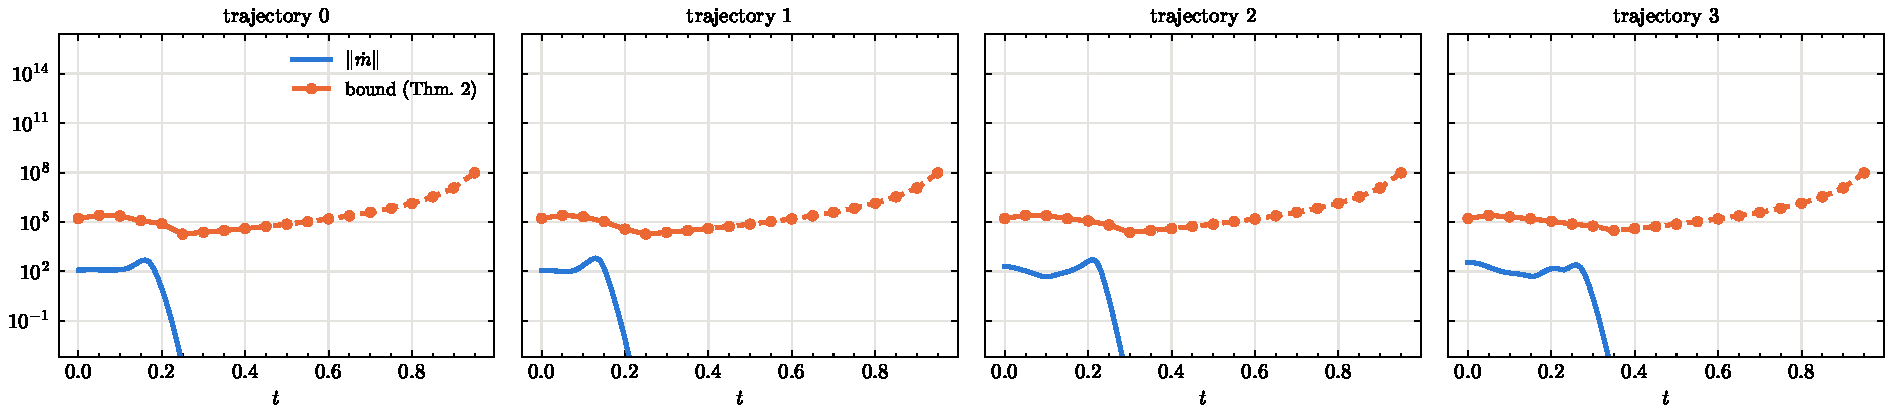
\includegraphics[width=\linewidth]{exact_field_cifar10/mdot_and_bound.pdf}
		\vspace{-0.4em}
		\begin{block}{How to read this (CIFAR-10, four sample paths, log scale)}
			\footnotesize \hl{Blue}: how fast the best guess moves, $\|\dot m\|$, i.e.\ how much the path bends. \hl{Orange}: our bound on it. The blue bump at $t \approx 0.13$ to $0.21$ is the moment the posterior commits to one image; afterwards $\|\dot m\|$ drops to $0$ and the path is straight. Across datasets, the peak coincides with commitment on $17$ of $24$ paths. The bound is always above the curve but $100$ to $5000$ times too large: it explains the shape, not the size.
		\end{block}
	\end{frame}

	\begin{frame}{Trained Networks Bend Differently}
		\centering
		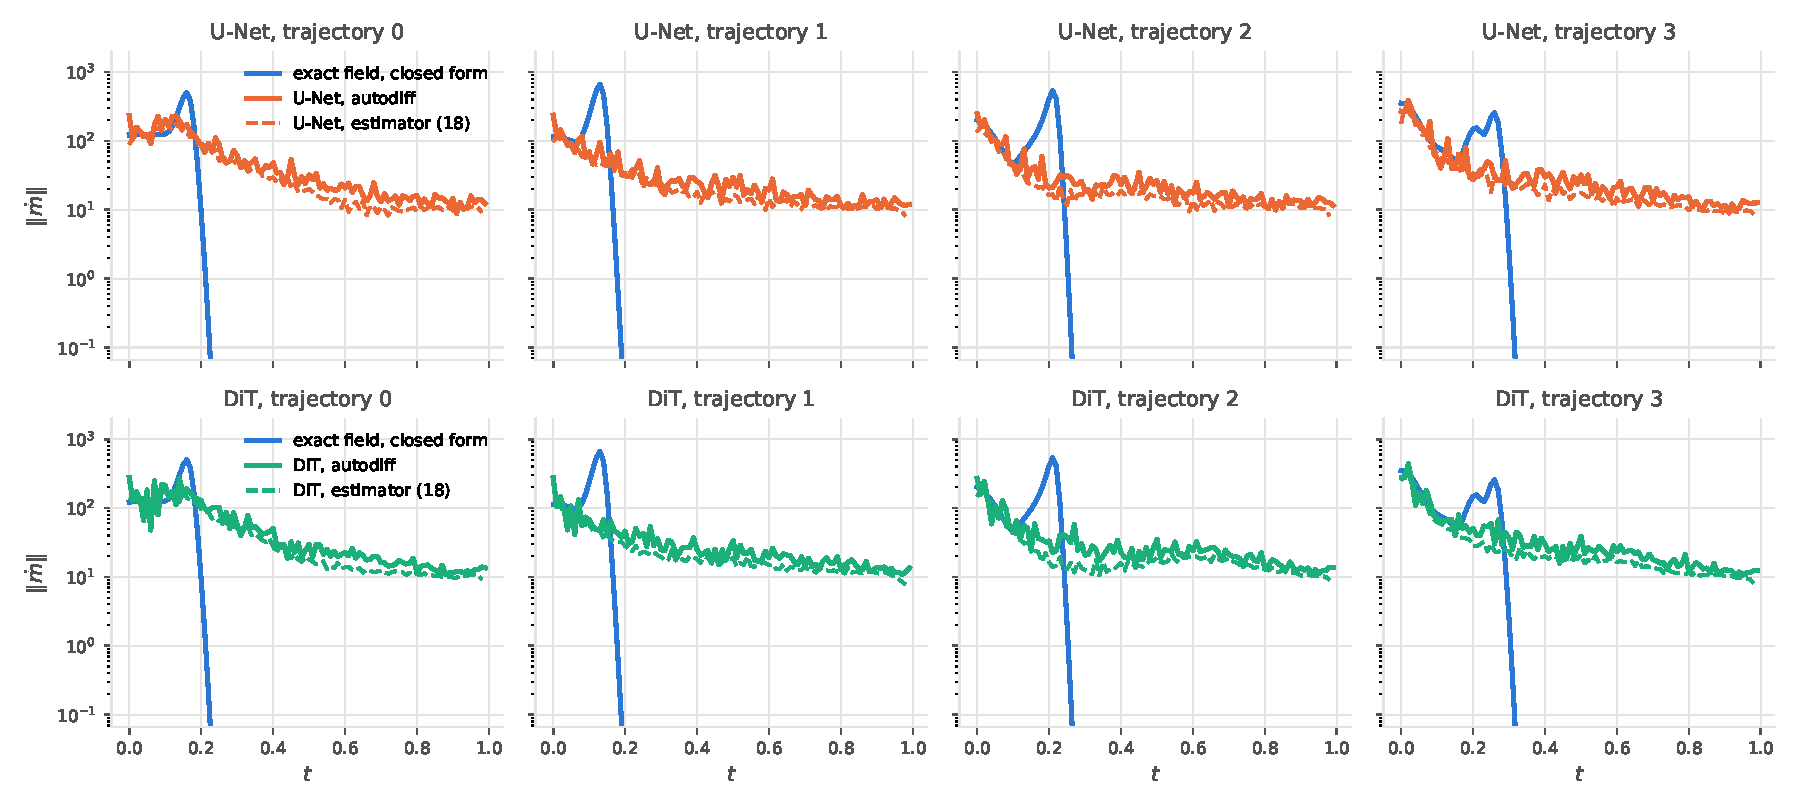
\includegraphics[width=0.74\linewidth]{trained_networks_cifar10/mdot_networks.pdf}
		\vspace{-0.6em}
		\begin{block}{How to read this (CIFAR-10, top U-Net, bottom DiT)}
			\footnotesize \hl{Blue}: bending of the exact field. \hl{Solid orange}: true bending of the network. \hl{Dashed}: our free estimate. Networks have \hl{no sharp peak} and keep bending mildly until the end: they do not commit to a training image, which is good, since the exact field only reproduces training images. The \hl{dashed line follows the solid one}, so the free estimate works on real networks.
		\end{block}
	\end{frame}

	\begin{frame}{Fewer Errors At The Same Cost}
		\centering
		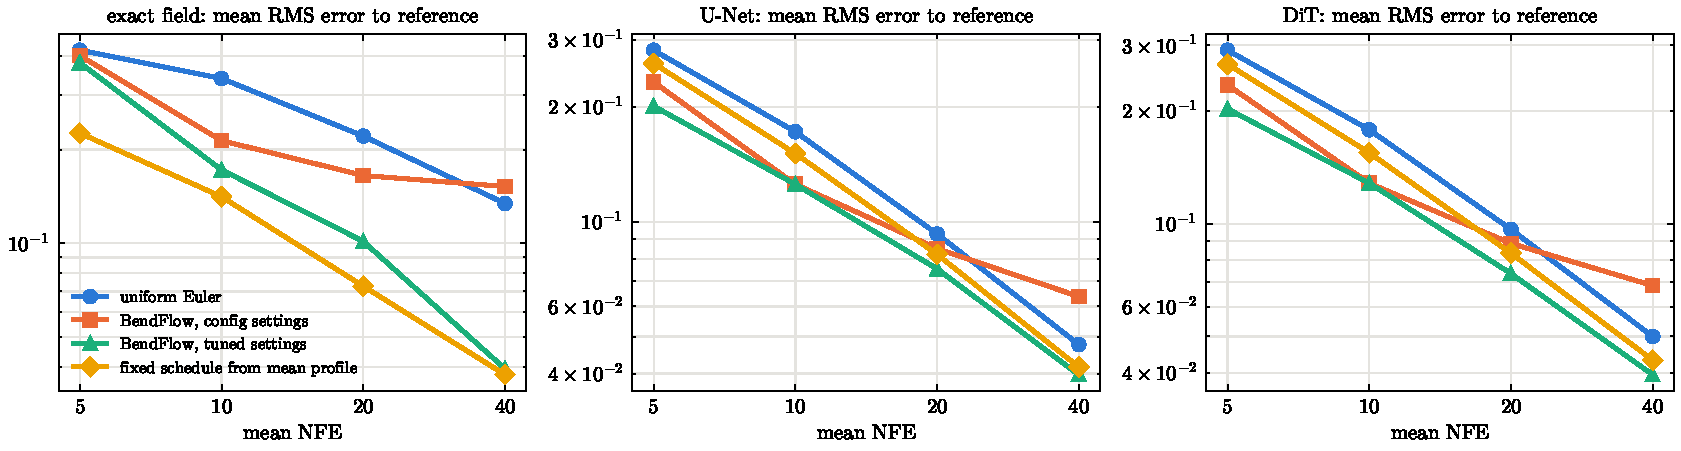
\includegraphics[width=0.86\linewidth]{schedule_baseline_cifar10_n128/error_vs_nfe.pdf}
		\vspace{-0.6em}
		\begin{block}{How to read this (CIFAR-10, log scales, lower is better)}
			\footnotesize x: network evaluations per sample. y: distance to the $1000$-step reference. \hl{Blue}: uniform Euler. \hl{Green}: BendFlow with settings tuned on separate samples. For both networks green is lowest everywhere, e.g.\ $0.125$ instead of $0.172$ at $10$ evaluations. \hl{Orange}, the untuned default, gets worse at $40$: the settings matter. \hl{Yellow}, one fixed schedule from the average bending, is best on the exact field.
		\end{block}
	\end{frame}

	\begin{frame}{Results At A Glance}
		\small
		How much smaller the error of tuned BendFlow is than that of uniform Euler with the same NFE ($-25\%$: a quarter less error; $+3\%$: slightly worse):
		\vspace{0.2em}
		\begin{center}
			\footnotesize
			\begin{tabular}{llcccc}
				\toprule
				Dataset & Network & NFE 5 & NFE 10 & NFE 20 & NFE 40\\
				\midrule
				MNIST & U-Net & $+3\%$ & $-3\%$ & $-9\%$ & $-9\%$\\
				 & DiT & $+3\%$ & $-3\%$ & $-9\%$ & $-15\%$\\
				Fashion-MNIST & U-Net & $-25\%$ & $-16\%$ & $-13\%$ & $-11\%$\\
				 & DiT & $-25\%$ & $-20\%$ & $-18\%$ & $-19\%$\\
				CIFAR-10 & U-Net & $-29\%$ & $-27\%$ & $-19\%$ & $-17\%$\\
				 & DiT & $-30\%$ & $-28\%$ & $-24\%$ & $-21\%$\\
				\bottomrule
			\end{tabular}
		\end{center}
		\vspace{0.2em}
		\begin{itemize}
			\item \hl{Biggest gains at few steps} and on the harder datasets.
			\item \hl{On MNIST} a single fixed schedule built from the average bending is as good or better.
			\item U-Net and DiT behave almost identically, although the DiT is four times larger.
		\end{itemize}
	\end{frame}

	\begin{frame}{What Does It Look Like?}
		\centering
		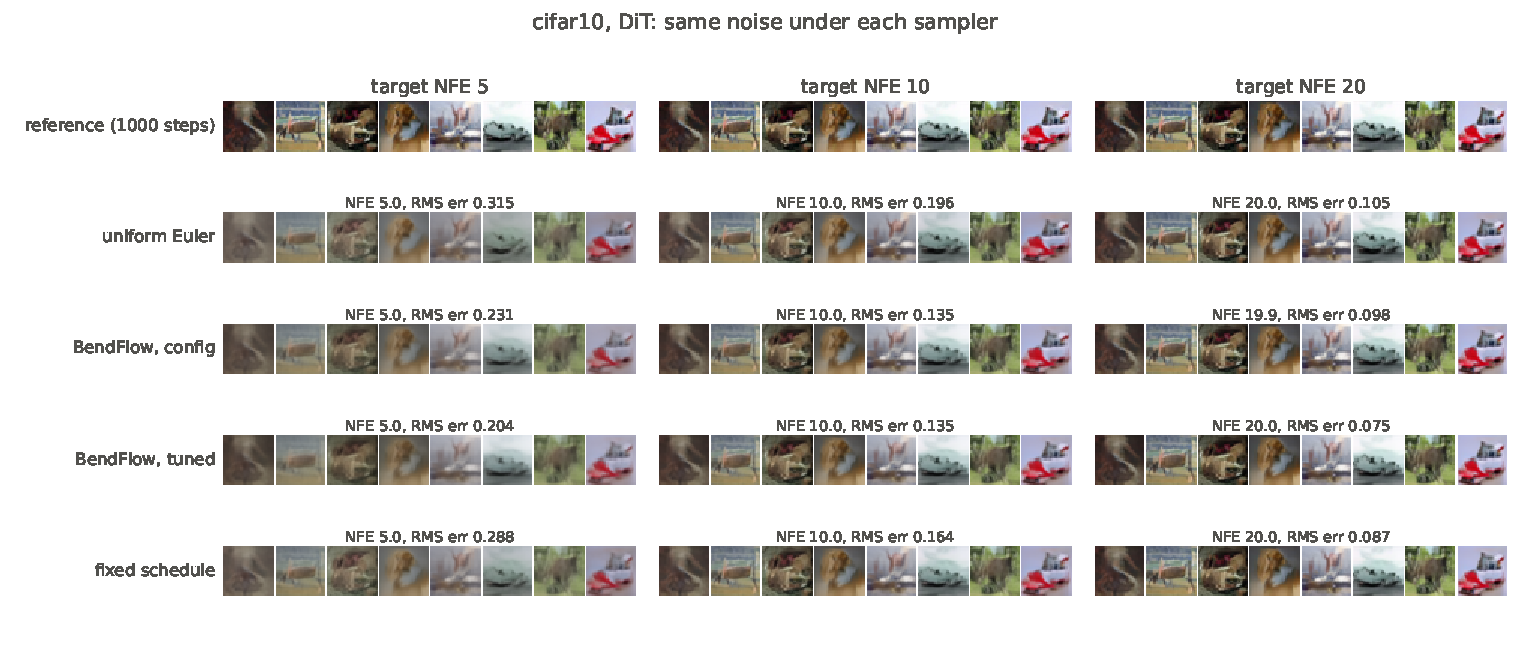
\includegraphics[width=0.82\linewidth]{sample_grids_cifar10/grid_dit.pdf}
		\vspace{-0.4em}
		\begin{block}{How to read this (CIFAR-10 DiT, same $8$ noise vectors in every row)}
			\footnotesize Top row: the $1000$-step reference. Each other row: one sampler at $5$, $10$ and $20$ evaluations, with its mean number of evaluations and error above the row. At $5$ steps every sampler is blurry; the tuned BendFlow row is closest to the reference. At $20$ steps all are close.
		\end{block}
	\end{frame}

	\begin{frame}{Takeaways And Limits}
		\begin{columns}[onlytextwidth, T]
			\begin{column}{0.48\textwidth}
				\begin{block}{What we learned}
					\footnotesize
					\begin{minipage}[t][4.0cm][t]{\linewidth}
						\begin{itemize}
							\item Bending has a closed form in terms of the posterior's spread and lopsidedness, for any Gaussian path.
							\item The exact field bends mostly when it commits to a training image.
							\item Real networks bend more smoothly, but the free estimate still tracks them.
							\item Curvature-based steps cut the error by up to $30\%$ at the same cost, once tuned.
						\end{itemize}
					\end{minipage}
				\end{block}
			\end{column}
			\begin{column}{0.48\textwidth}
				\begin{block}{What we did not show}
					\footnotesize
					\begin{minipage}[t][4.0cm][t]{\linewidth}
						\begin{itemize}
							\item The bounds on $\kappa$ and $\dot m$ are too loose to use as numbers.
							\item Default settings can lose to uniform Euler; tuning is needed.
							\item Experiments only on the linear path; small networks, $128$ samples, one draw of noise.
							\item Error to a reference, not sample quality.
						\end{itemize}
					\end{minipage}
				\end{block}
			\end{column}
		\end{columns}
	\end{frame}

	\begin{frame}[plain]
		\centering
		\vfill
		{\fontsize{40}{48}\selectfont\textcolor{coolpurple}{\textbf{Questions?}}}
		\vfill
	\end{frame}

\end{document}
